\documentclass{article}
\begin{document}

\title{CrowdEgress: A Multi-Agent Simulation Tool for Crowd Evacuation}

\maketitle

\section{Introduction} 

The program mainly consists of four component: User Interface, Simulation Core, Data Tool, Visualization Tool

\textbf{User Interface}: The user interface is written in tkinter in ui.py.  Please run ui.py to enable a graphic user interface (GUI) where one selects the input files, initialize compartment geometry, and configure or start a simulation.  An alternative method is using evac-non-gui.py to directly start a simulation without GUI.  Currently there is a simple version of GUI and it needs to be improved in several aspects.  

\textbf{Simulation Core}: The multi-agent simulation is implemented in simulation.py.  The component is packed in a class called simulation class, and it computes interaction of four types of entities: agents, walls, doors and exits.  The agent model is described in agent.py, while walls, doors and exits are coded in obst.py.  The agent-based model is an extension of the traditional social force model by Helbing, Farkas, Vicsek and Monlar.  The model aims at investigating protypes of pedestrian behavior in crowd evacuation.  The core algorithm is still being studied and developed.  This is an interesting study topic, which refers to Newton particles, complex systems and behavioral science.  Your comments or contribution are much welcome.  

\textbf{Data Tool}: This component reads in data from input files, and write data to output files.  The input data is written by users in .csv files.  Agents and exits must be specified in .csv file while walls and doors can be described either in .csv file or read in from standard .fds input file.  In the future.  We may plan to use a subroutine in FDS+Evac to output the agent movement data so that the agent movement can also be visualized by smokeview. 

\textbf{Visualization Tool}: The visulization component is packed in draw\_func.py and currently pygame (SDL for python) is used to develop this component.  Currently simulation is started and visualized in the meantime.  In the future we may set them apart such that users first run the simulation and get the output data, and then visualize the data.  If any users are interested, please feel free to extend the module or try other graphic libraries to wrtie a visulization component.


\section{About Simulation Model}

Agent-based model (ABM) describes interactions among individual agents and their surroundings.  In the simulation core there are four types of entities: agents, walls, doors and exits, and their interactions are illustrated in Figure 1.  

\begin{figure}
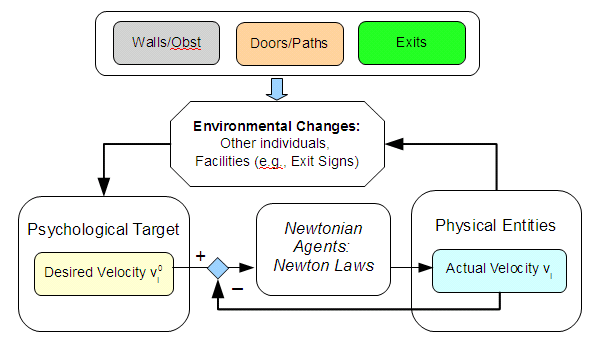
\includegraphics[bb=0bp 0bp 595bp 342bp,clip,scale=0.43]{img/NewtonLaw01}
\caption{Figure1. Simulation Model: Interaction of Newtonian Agents and Their Surroundings}\label{Fig_SimulationModel}
\end{figure}

\textbf{Walls}: Walls are obstruction in a compartment geometry that confine agent movement, and they set up the boundary of a room or certain space.  Just like walls in normal buildings, walls may be labeled with arrows that direct agent to move toward certain directions.  In our program wall are either lines or rectangular areas.  If any users are interested, please feel free to extend the wall types to circular or polyangular areas.

If users specify a line obstruction, it is expected to input the position of starting point and ending point of a line.  If users specify a rectangular obstruction, it is required to input the position of upper left point and lower right point of a line.  

start X: x position of starting point for line obstruction; x position of upper left point for rectangular obstruction.  
start Y: y position of starting point for line obstruction; y position of upper left point for rectangular obstruction.  
end X: x position of ending point for line obstruction; x position of lower right point for rectangular obstruction.  
end Y: y position of ending point for line obstruction; y position of lower right point for rectangular obstruction.  
mode: either line or rectangular obstruction in current program
id: id number assigned to this obstruction; id number is optionally shown in the pygame screen so that users can easily modify the obstruction
inComp: a boolean variable to indicate if the obstruction is in computation or not
arrow: direction assigned to the obstruction so that agents will be guided when they do not have any target door or exit 

\textbf{Doors}: Doors are passageways that direct agents toward certain areas, and they may be placed over a wall so that agents can go through the wall by the door.  Doors can also be placed as a waypoint if not attached to any walls, and they can be considered as arrows or markers on the ground that guide agent movement.  In brief doors affect agent way-finding activities and they help agents to form a roadmap to exits.  In current program doors are only specified as rectangular areas.

\textbf{Exits}: Exits are a special types of doors which finally evacuate agents to the safety.  Thus they may be considered as safety areas, and computation of an agent terminates when the agent reaches the exits.  An exit is usually placed over a wall like doors, but it can also be put anywhere independently without walls.  Exits must be specified in .csv file.  In the program exits are only defined as rectangular areas.

\textbf{Agents}: Finally and most importantly, agents are the core entity in computation.  They interact with each other to form collective behavior of crowd.  They also interact with above three types of entities to form egress motion toward exits.  The resulting program is essentially a multi-agent simulation of pedestrian crowd.  Each agent is modeled by extending traditional social force model.  The model is further advanced by integrating several features including pre-evacuation behavior, group behavior, way-finding behavior and so forth.


\section{How-To}

\textbf{In Tkinter Screen}: When tkinter window (GUI) is activated, please select the input files for simulation.  Choose .csv file for evac input data.  Users can optionally use .fds file to create the compartment geometry, and the pedestrian features are described in .csv file.  If both .csv and .fds files are presented, the compartment structure will be created by using .fds file.  If .fds file is omitted, the compartment geometry is described in .csv file.  The agents and exits must be specified in .csv file currently while the walls and doors can either described by .csv file or .fds file.  Please take a look at the examples for details.

\begin{figure}
\centerline{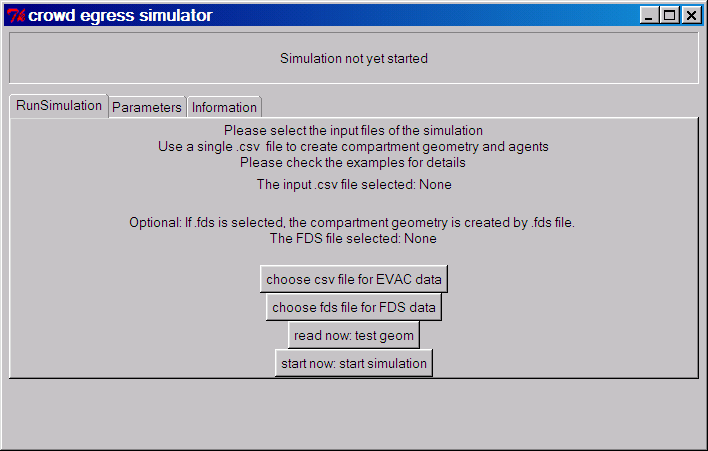
\includegraphics[bb=0bp 0bp 595bp 342bp,clip,scale=0.43]{img/gui}}
\caption{In Tkinter Screen}\label{Fig_TkScreen}
\end{figure}


\textbf{In Pygame Screen}: When pygame screen is displayed, press keys to adjust the display features and visualize entity data.
Use pageup/pagedown to zoom in or zoom out the entities in screen
Use space key to pause the simulation
Use arrows to move the entities vertically or horizonally in screen.
Use 1/2/3 in number panel (Right side in the keyboard) to display the door or exit data on the screen.

There are two sections in pygame screen.
One section is TestGeom, where users can visualize geometric settings and modify them manually.  Users can also dump geometric data (e.g., wall data and door data) into .csv file by selecting the items in the menu bar.

The other section is RunSimulation, in which the evac simulation is started and visualized on the screen.  User can pause the simulation, but cannot rewind it in current version (Version 2.0)

\textbf{Try Examples}: There are currently two examples in the repo.  Please execute run.bat in the subfolders to run the example.  The examples are run by using non-gui method.  Users can also learn how to write the .csv files from the examples.

\end{document} 